\documentclass[a4paper, 11pt]{memoir}

\usepackage[francais]{babel}
\usepackage[T1]{fontenc}
\usepackage[utf8]{inputenc}

\usepackage{amsmath,amsfonts,amssymb} % Pour les formules mathématiques

\usepackage{float}
\usepackage{graphicx} % pour les images

\usepackage[bookmarks,hidelinks]{hyperref}

\title{
  \huge{SoundCity} \\
  Génération de playlist de qualité \\
  Projet de Programmation
}
\author{Lucas Vauzelle \and Baptiste Fumaroli \and Jean Pecqueur \and Thomas Pizon}
\date{\today}

\setsecnumdepth{subsubsection}
\setcounter{tocdepth}{3}

\begin{document}

\maketitle % Page de titre
\clearpage

\frontmatter*

\chapter*{Introduction}

De nombreux générateurs de playlists existent (en ligne pour la plupart), mais
les playlists générées ressemblent plus à une sélection intelligente ordonnée
n'importe comment, plutôt qu'à une playlist de soirée crée par un DJ. À travers
ce projet, nous voulons proposer un outil qui ne se limite pas à un filtrage
d'une quelconque base de données. Nous voulons créer des ensembles cohérents de
morceaux, qui s'enchaînent sans cet effet de rupture qui est souvent présent
dans les services de playlists, ou dans les playlists aléatoires.

Notre but est donc de fournir des playlists de qualité, issues de contenus
filtrés ou totalement aléatoires, en jouant sur leur ordre.

Mais qu'est ce qui permet de juger la qualité d'un playlist, et quels moyens
a-t-on à notre disposition pour comparer des morceaux musicaux~?

\clearpage

% Table des Matières
\tableofcontents

\mainmatter*

\chapter{Étude de l'existant}

\section{Qualité d'une playlist}
\label{existant:qualite}

Les conférenciers Ben Fields et Paul Lamere ont présenté une très bonne
conférence \cite{ismir2010:playlist-tutorial} qui constitue une bonne approche
de la construction de playlists.

Ils définissent la playlist comme étant un ensemble de morceaux \emph{ordonnées}
\cite[p.~7]{ismir2010:playlist-tutorial}. L'ordre des morceaux est donc
important.

Il décrivent une playlist de qualité comme étant influencé par un certains
nombre de facteurs \cite[p.~17--18]{ismir2010:playlist-tutorial}. Le facteur qui
nous intéresse majoritairement est le «~niveau de variété et de cohérence~» de
la playlist.

La \emph{cohérence} est présentée \cite[p.~21 -- 23]{ismir2010:playlist-tutorial}
comme une aide à la construction de mix permettant de rapprocher les morceaux.
La paramètre de cohérence qui nous intéresse ici est la «~Song Similarity~» qui
définit la similarité entre des morceaux en analysant le signal audio.
Les Paramètres «~Artist / Genre / Style~» sont aussi important mais relèvent du
contexte du morceau.

Une autre composante importante est la \emph{variation} 
\cite[p.~32]{ismir2010:playlist-tutorial}. En effet une cohérence trop forte
dans une playlist provoquera une certaine monotonie. Il faut donc éviter cela
en prenant en compte la variation dans la qualité de la playlist.

\section{Générateurs de playlists existants}
\label{existant:generateurs}

\subsection{Musicovery}
\label{existant:musicovery}

Musicovery est un site web qui propose une lecture en streaming d'une 
playlist de morceaux musicaux, qui sont sélectionnés selon plusieurs types 
de paramètres, qui peuvent être combinés afin d'affiner la recherche.

En effet, le site propose d'effectuer des recherches par artiste, par tag, 
par année, ou par genre. Mais son originalité réside en un placement des 
morceaux dans un graphique en deux dimensions selon les deux axes suivants:
sombre/positif et énergique/calme.
Ainsi, chaque utilisateur de ce site peut écouter une playlist de morceaux 
variés et d'artistes différents, tout en restant dans le même thème, selon 
son humeur du moment.
En plus de cela, l'utilisateur peut demander une playlist de musiques plus 
ou moins connues et populaires grâce aux deux options "Hits" et "Découverte".

Le site propose également quelques options supplémentaires comme le partage 
sur les réseaux sociaux, ou encore une inscription afin de garder en mémoire 
des morceaux favoris.

http://musicovery.com/

\subsection{Spotibot}
\label{existant:spotibot}

Spotibot est un site internet permettant de créer une playlist en fonction 
d'un nom d'artiste rentré par l'utilisateur (ou de plusieurs), ou alors en 
se basant sur son profil Last.fm. Comme le nom du site peut le laisser 
penser, la lecture de la playlist ainsi générée est effectuée sur Spotify.

Sur ce site, les options et les précisions que peut faire l'utilisateur sont 
assez limitées. En effet, il peut uniquement choisir la taille de la 
playlist demandée (en nombre de morceaux), et si il préfère avoir des 
morceaux populaires ou non.

Une fois que l'utilisateur a validé sa recherche, Spotibot lui renvoie une 
playlist du nombre de morceaux demandé, en fonction de la similarité avec 
l'artiste saisi (via les tags, et via l'historique des écoutes du compte 
Last.fm). Une fois cette playlist générée, l'utilisateur peut décider d'y 
ajouter quelques morceaux supplémentaires à l'aide d'un simple bouton, ou 
alors d'enlever des morceaux qui ne lui conviennent pas.

Une fois finalisée, la playlist peut être exportée pour être lue directement 
sur Spotify par simple Drag'n'Drop.

Ce site possède également un top des groupes/artistes les plus populaires et 
les plus recherchés, mais aussi de ceux les plus supprimés.

http://www.spotibot.com/

\subsection{Sourcetone}
\label{existant:sourcetone}

Sourcetone est une application qui permet de classer des morceaux d'une 
bibliothèque musicale en différentes catégories, afin avoir des playlists 
correspondant à l'humeur et/ou à l'activité du moment. Par exemple, cela 
permet d'avoir une playlist entraînante pour faire du sport, ou une playlist 
plus calme pour se reposer le soir.

Sourcetone possède également une fonction radio, que l'utilisateur peut 
paramétrer selon ses envies (musique rythmée ou non, joyeuse ou non, de 
quelle année, etc.).

L'application se base sur les évaluations et les avis de l'utilisateur 
lui-même: elle a besoin d'un retour, dans le but "d'apprendre" à mieux le 
connaître, afin de lui proposer des musiques de plus en plus adaptées selon 
son humeur ou son activité.

http://www.sourcetone.com/ % Etude de l'existant

\chapter{Objectifs}

\section{Objectifs}
Comme il est expliqué plus haut, plusieurs générateurs de playlists existent
déjà, et permettent de fournir une sélection de morceaux articulée autour 
d'un même thème et de plusieurs paramètres.
Notre objectif principal est de générer une playlist selon les mêmes types 
de critères, en gardant une cohérence globale, mais en attachant une 
importance particulière à l'enchaînement des morceaux. Ainsi, les morceaux 
de la playlist générée par SoundCity se suivent selon un ordre optimal afin 
d'éviter des transitions brutales entre deux musiques qui correspondent aux 
criètres de recherches rentrés, mais qui sont trop différents dans leur 
structure musicale (tempo trop différent, époque trop lointaine, etc.).

Pour effectuer la génération de la playlist, l'utilisateur a la possibilité 
d'entrer des paramètres afin d'influencer et de préciser la création de la 
suite de morceaux. Il pourra ainsi sélectionner une tranche d'années s'il le 
souhaite, ou encore un artiste autour duquel articuler l'élaboration de la 
playlist.

L'originalité et l'apport supplémentaire qu'offre SoundCity par rapport aux 
autres générateurs est donc l'enchaînement des morceaux. La partie centrale 
du logiciel est celle qui s'occupe d'ordonner les musiques sélectionnées 
dans la base de données. En effet, la sélection des morceaux correspondants 
aux données rentrées par l'utilisateur n'est qu'un filtrage, tandis que 
l'ordonnancement se concentre sur la similarité de ces musiques afin de les 
faire s'enchaîner au mieux.

La base de donnée utilisée pour le logiciel est tirée de la Million Song 
Dataset (MSD). Comme son nom l'indique, c'est une base de données d'un 
million de morceaux musicaux, qui contient toutes les informations 
nécessaires sur les musiques, et dont la fiabilité est assurée.

Un autre point important que le logiciel doit avoir, c'est le retour 
utilisateur (feedback). La génération de la playlist peut prendre jusqu'à 
plusieurs dizaines de secondes, et pendant ce temps là, il ne faut pas 
laisser l'utilisateur sans aucune information. Pour ce faire, à tout moment 
de la génération, une simple information sur le nombre de morceaux ajoutés à 
la playlist à cet instant est affichée à l'utilisateur. % Objectifs du PdP

\chapter{Analyse des besoins}
\section{Analyse des besoins fonctionnels}
\label{besoins:fonc}

\subsection{Génération de Playlist}
\label{besoins:fonc:generation}

L’objectif principal de ce projet est de générer une playlist cohérente de 
morceaux en fonction des paramètres rentrés par l’utilisateur. Cette génération 
se décompose en 2 parties distinctes.

\subsubsection{Sélection: interaction avec les données}
\label{besoins:fonc:generation:selection}

Lors de l’étape de sélection, le programme doit être capable de choisir un 
ensemble de morceaux qui correspondent aux paramètres voulus par l'utilisateur, 
tous étant optionnels. Cet ensemble est appelé la «~Pool de morceaux~». Dans le 
cas où aucune de ces options n’est fixée, la sélection des pistes doit se faire 
de manière aléatoire.

\vspace{3mm}
\noindent Les paramètres sont les suivants~:
\begin{itemize}
\item La durée de la playlist voulue, en nombre de morceaux.
\item Le nom d'un artiste/groupe.
\item Une tranche d'années.
\item Un score de popularité.
\end{itemize}

\vspace{3mm}
\noindent À ces données, on en ajoute trois basées sur le signal~:
\begin{description}
\item[Rythme~:] étant calculé d'après le tempo.
\item[Énergie~:] pouvant être calculée à partir du paramètre de «~loudness~».
\item[Humeur~:] pouvant être calculée en fonction de la tonalité du morceau 
(Note~: l’humeur n’est pas nécessairement une donnée basée sur le signal. En 
effet, le client peut très bien fournir cette information en recueillant des 
avis de personnes diverses).
\end{description}

Ces informations sont considérées comme étant exactes et fiables. Dans la base 
de données, elles sont toutes stockées dans des nombres flottants compris entre 
0 et 1. Cependant, le créateur d'une nouvelle base de données est libre 
d'imposer sa propre convention pour le calcul de ces valeurs.

\subsubsection{Ordonnancement: Similarité entre les morceaux}
\label{besoins:fonc:generation:selection:ordonnancement}

Lors de l'ordonnancement, les pistes placées dans la Pool de morceaux doivent 
être agencées tout en respectant une certaine cohérence, mais également une 
variété. Un score de similarité est donc calculé entre les différents morceaux 
afin de repérer ceux qui sont les plus semblables.

Ce calcul doit donner un score de similarité entre deux pistes. Une playlist 
cohérente est donc une playlist dans laquelle chaque morceau possède un score 
de similarité élevé avec le morceau qui le précède et celui qui le suit.

\subsection{Visualisation de la playlist}
\label{besoins:fonc:generation:visu}

La playlist ainsi crée doit pouvoir être utilisable après avoir été générée. 
Il faut donc un moyen de la visualiser, et possiblement, de l’écouter. Le 
moyen le plus simple, mais le plus rudimentaire, est le format textuel. Ce 
format de sortie est principalement utilisé pour les tests, son utilité étant 
réduite dans les autres cas.

Un second moyen de visualiser, ou plutôt d'écouter la playlist, est d’utiliser 
un service de streaming. Celui qui a retenu notre attention est Deezer, car son 
API est en accès libre et que la construction d'une playlist est assez simple. 
Il suffit en effet d’utiliser une API javascript.
        
\subsection{Interface Utilisateur et feedback}
\label{besoins:fonc:generation:feedback}

Pour interagir avec le générateur, l’utilisateur doit passer par une interface 
(qu'elle soit graphique, ou en console) permettant de paramétrer le dit 
générateur. De plus, il est important d’envoyer un feedback des actions 
réalisées par le programme à l’utilisateur. Il faut donc utiliser un système 
nous permettant de visualiser l’avancement de la génération.

\section{Analyse des besoins non fonctionnels}
\label{besoins:nfonc}

\subsection{Performances}
\label{besoins:nfonc:perf}

Les performances lors de la génération de la playlist sont importantes, car nous
voulons éviter de frustrer les utilisateurs avec un temps d'attente trop long.

Le feedback de l’interface permet de faire patienter, mais il faut aussi 
raisonner en performance brute. Le nombre de pistes qui correspondent aux 
critères rentrés par l’utilisateur peut être énorme. Il faut donc filtrer et 
limiter le nombre de ces résultats, tout en conservant une le caractère 
aléatoire de la sélection.

Nous avons donc décidé de limiter le nombre de morceaux sur lesquels faire nos 
calculs et notre ordonnancement. Les pistes sélectionnées étant un 
sous-ensemble plus petit de tous les morceaux correspondant aux critères 
choisis, notre convention est donc de limiter ce sous-ensemble de pré-sélection 
à 10 fois la taille de playlist demandée par l’utilisateur. Ainsi, pour une 
génération de 15 morceaux, une pré-selection de 150 morceaux est effectuée, 
et la génération se fait uniquement à partir de ces morceaux. Ce système permet 
de limiter la complexité d'une génération car chaque morceau de la Pool est 
comparé à tous les autres, et ce, à chaque insertion d'une nouvelle piste dans 
la playlist. La complexité est donc de \[O(n) = n*(n*10)\], n étant la taille 
de la playlist générée.

\subsection{Modularité}
\label{besoins:nfonc:perf:mod}
    
Le projet se doit d'avoir chacune de ses parties indépendantes et remplaçables 
à souhait. Pour cela, le programme est séparé en 4 modules~:

\subsubsection{Module d'Interface Utlisateur}
\label{besoins:nfonc:perf:mod:iu}

(c.f. Section \ref{besoins:fonc:generation:feedback})

\subsubsection{Module de génération de playlist}
\label{besoins:nfonc:perf:mod:generator}

Ce module est chargé de générer la playlist en fonction d’un panel de 
descripteurs de morceaux et de paramètres. Il s'agit de la partie 
d'ordonnancement. Il est lié au module de données (c.f. Section 
\ref{besoins:nfonc:perf:mod:data}) qui se charge de la sélection des morceaux.

\subsubsection{Statégie de similarité}
\label{besoins:nfonc:perf:mod:similarity}

Ce module utilise le pattern Strategy afin de le rendre interchangeable. Cette 
classe, qui est uniquement appellée par le module de génération, contient une 
fonction qui calcule le score de similarité entre deux morceaux passés en 
paramètres.

\subsubsection{Module de données}
\label{besoins:nfonc:perf:mod:data}

Cette partie est chargée de récupérer les données pour alimenter le générateur. 
Elle peut être changée en fonction du type de données à lire (fichier(s), 
base(s) de données, etc). Nous n'avons fait qu’un seul module qui travaille 
sur une base de données SQL.

\subsubsection{Module de sortie}
\label{besoins:nfonc:perf:mod:out}

Il peut y avoir plusieurs modules de sortie s'imbriquant dans le programme, mais
il en faut au minimum un. Ce module se charge de convertir, puis de rendre à
l’utilisateur, la playlist (déjà générée par le module de génération) au 
format souhaité.

\begin{figure}[H]
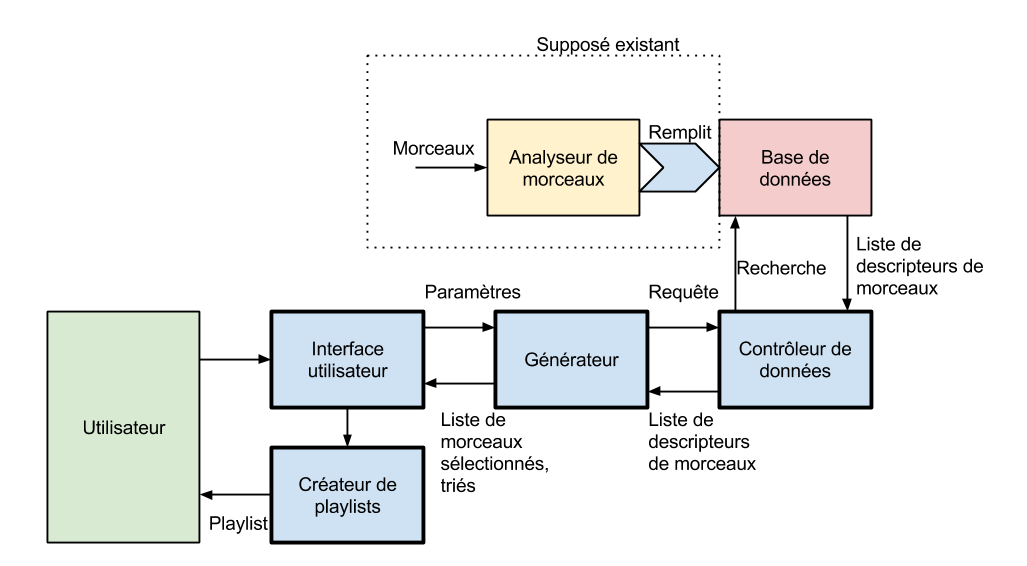
\includegraphics[width=\textwidth]{data/besoins/modules.png}
\caption{Les 4 modules indispensables au bon fonctionnement du programme et leurs
interactions.}
\end{figure}

\subsection{Ergonomie}
\label{besoins:nfonc:perf:erg}
Les interfaces doivent être utilisables par un utilisateur non-avancé et éviter 
de le perdre en étant claires et précises. Les termes employés sur cette 
interface sont donc écrits dans un vocabulaire compréhensible par tous, sans 
utiliser de mots ou d'expressions trop techniques.

\section{Contraintes}
\label{besoins:contraintes}

\subsection{Base de données}
\label{besoins:contraintes:bdd}
Nous ne disposons pas d’analyseur de morceaux, et en créer un ne fait pas partie
de notre sujet. Nous devons donc utiliser nous-même une base de données déjà
existante afin de travailler dessus. Nous avons donc choisi d’utiliser la Million
Song Dataset (http://labrosa.ee.columbia.edu/millionsong/) qui contient toutes
les informations dont nous avons besoin. Nous avons dû la convertir en base de 
données SQL afin d'améliorer le temps de récupération des données. Il nous a 
donc fallu comprendre le fonctionnement de la MSD dans le but d'écrire un 
script qui nous a permis d'en extraire les informations nécessaires pour notre 
programme et créer une base de données SQL.
    
Cette base de données pèse 500 Go, et la conversion double la place nécessaire 
pour stocker notre base de données. Bien que nous travaillons sur un 
échantillon restreint au départ, nous devons disposer d’un espace de travail 
d’au moins 1 To. Nous avons donc travaillé sur cet échantillon pour un gain de 
temps, de convertion, et de stockage.

La MSD est la seule base pouvant nous servir de test, et les informations 
qu'elle contient sont parfois très inexactes voire complétement absentes. Nous 
devons faire abstraction de ces cas particuliers, même si ils peuvent nous 
poser des problèmes dans le cadre des tests (puisque nous considérons les 
informations comme complètes et exactes).

La base de données que nous utilisons au final sera donc une conversion en base 
SQL de la Million Song Database, dont nous avons extrait uniquement les valeurs 
dont nous avons besoin.

\section{Prototypes}
\label{besoins:proto}

\subsection{Interface utilisateur graphique}
\label{besoins:proto:gui}
    
L'idée de notre interface graphique est de permettre à un utilisateur non aguérri
de faire fonctionner notre programme sans avoir de grandes connaissances en
informatique musicale. C'est pourquoi nous avons choisi de réaliser une interface
graphique simple, et au vocabulaire accessible. Par exemple, l'energie du morceau
est représentée par un curseur pouvant varier de «~léger~» à «~puissant~», sans
proposer à l'utilisateur de choisir une valeur numérique précise, ce qui ne
représenterait rien à ses yeux.
    
Les différents paramètres d'entrée sont ainsi organisés de façon à partir du plus
basique au plus complèxe, en regroupant les paramètres dits contextuels (artiste,
genre etc.) en haut, et les desripteurs audio en dessous (rythme, énergie, etc.).

Enfin nous proposons d'inclure des checkboxs afin que l'utilisateur puisse
choisir quels paramètres il veut prendre en compte, et ainsi lui laisser
la possibilité de choisir le niveau de spécification de la playlist.
    
\begin{figure}[H]
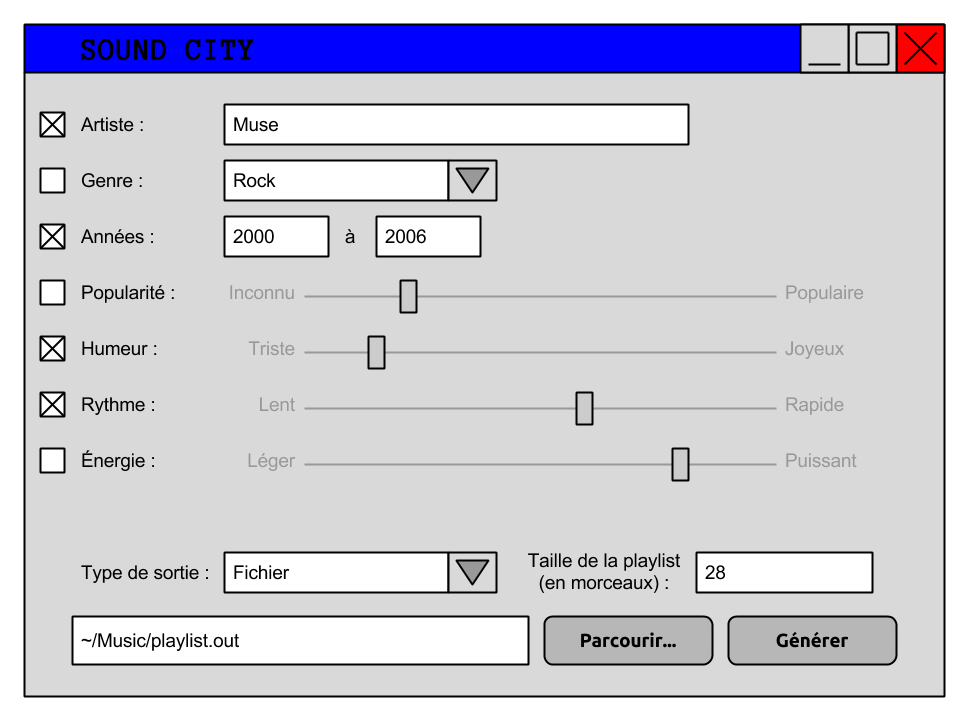
\includegraphics[width=\textwidth]{data/besoins/interface_utilisateur.png}
\caption{Prototype de l'interface utilisateur graphique.}
\end{figure}

\subsection{Interface utilisateur console}
\label{besoins:proto:console}

Cette interface possède les mêmes fonctionnalités que l'interface graphique, à 
la différence que tous les options sont placées lors de l'exécution programme :

\vspace{3mm}
\noindent Les paramètres sont les suivants~:
\begin{itemize}
\item \texttt{-y <startYear[1-3000]> <endYear[1-3000]>} : Définit un intervalle 
d'années pour les morceaux.
\item \texttt{-e <energy[0.0-1.0]>} : Impose une valeur d'énergie dans 
la playlist générée.
\item \texttt{-p <popularity[0.0-1.0]>} : Impose une valeur de popularité 
dans la playlist générée.
\item \texttt{-r <rhythm[0.0-1.0]>} : Impose un rythme dans la 
playlist générée.
\item \texttt{-m <mood[0.0-1.0]>} : Impose une humeur dans la 
playlist générée (plus la valeur est élevée, plus le morceau est joyeux).
\item \texttt{-s <size[1-100]>} : Choix de la taille de la 
playlist générée (10 par défaut).
\item \texttt{-o <fileName>} : Choix du nom du fichier de sortie.
\item \texttt{-a <artistName>} : Impose un artiste.
\end{itemize}
 % Analyse des besoins

\chapter{Scénarii d'utilisation}

\section{Initialisation du programme}
\label{scenarii:init}
    
Lors de l'initialisation du programme, trois cas de figure peuvent être
rencontrés : 

\begin{itemize}
\item L'initialisation se passe correctement et le programme est prêt à être
utilisé.
\item Une erreur est introduide à cause d'un échec de connexion à la base de
données.
\item Une erreur est introduite à cause d'un échec de connexion au module de
sortie.
\end{itemize}

\subsection{Initialisation réussie}
\label{scenarii:init:reussie}

Lors du démarrage du programme, l'interface utilisateur va demander au 
module de génération de playlists de vérifier la présence d'une base de 
données accessible. La rêquete est alors transmise du générateur au module 
de données qui va effectuer une connexion avec la base de données.
        
Une fois cette connexion correctement effectuée, le module de données va 
faire remonter l'information au générateur qui va, à son tour, la 
transmettre à l'interface utilisateur.

Ensuite, l'interface utilisateur s'assure qu'il y ait au moins un module de 
sortie fonctionnel en récuperant une liste des différentes sorties possibles.

Enfin, l'interface utilisateur s'adapte pour correspondre aux services de 
sortie disponibles.
        
\begin{figure}[H]
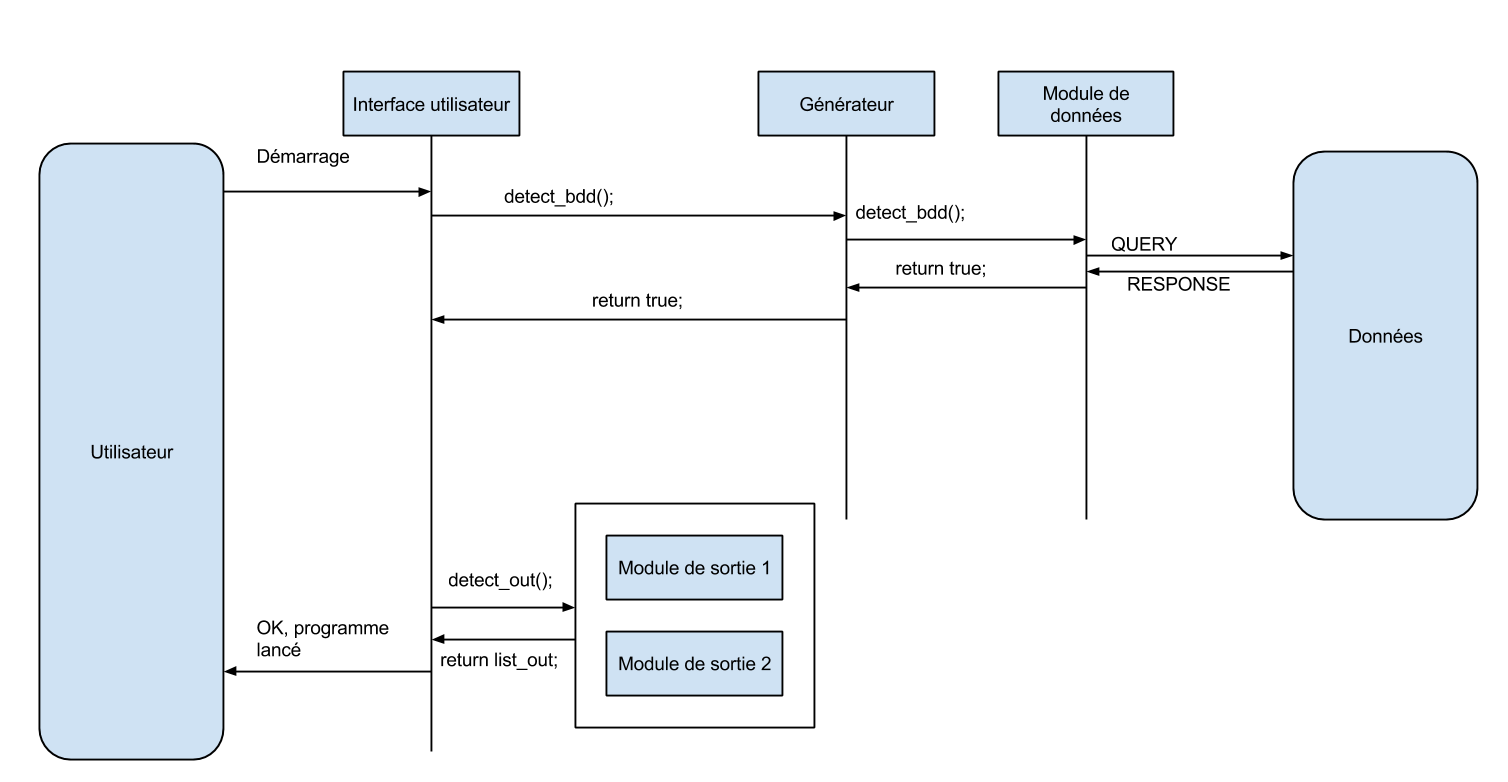
\includegraphics[width=\textwidth]{data/scenarii/demarrage_fonctionnel.png}
\caption{Initialisation réussie, le programme est lancé.}          
\end{figure}
        
\subsection{Absence de base de données}
\label{scenarii:init:nobdd}
        
Lorsque le module de données tente de se connecter à la base de données, il 
se peut que la connexion échoue pour diverses raisons. Dans ce cas, le 
module de données renvoie au générateur un message d'erreur qu'il transmet à
 l'IHM, afin de l'afficher pour avertir l'utilisateur de cette erreur. Puis 
 le programme s'arrête.
        
\begin{figure}[H]
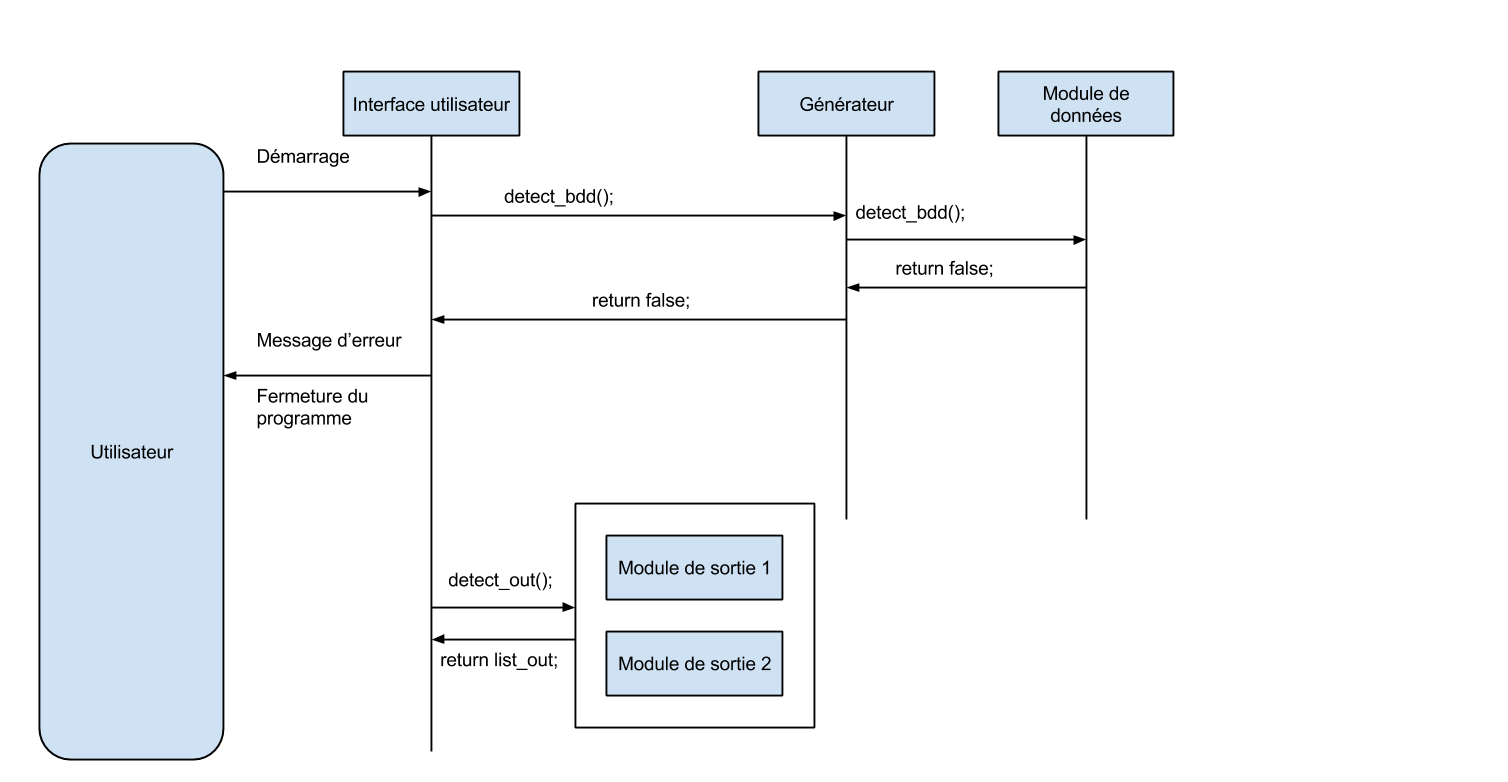
\includegraphics[width=\textwidth]{data/scenarii/demarrage_absence_bdd.png}
\caption{Absence de base de données lors de l'initialisation}
\end{figure}
        
\subsection{Absence de module de sortie}
\label{scenarii:init:noout}

Dans le cas où l'interface utilisateur effectue correctement une connexion à 
la base de données, mais n'arrive pas à établir une liste des sorties 
disponibles (à cause d'une absence du module de sortie ou d'aucune sortie 
disponible), elle doit afficher un message d'erreur à l'attention de 
l'utisilateur, et entraîner l'arrêt du programme.
        
\begin{figure}[H]
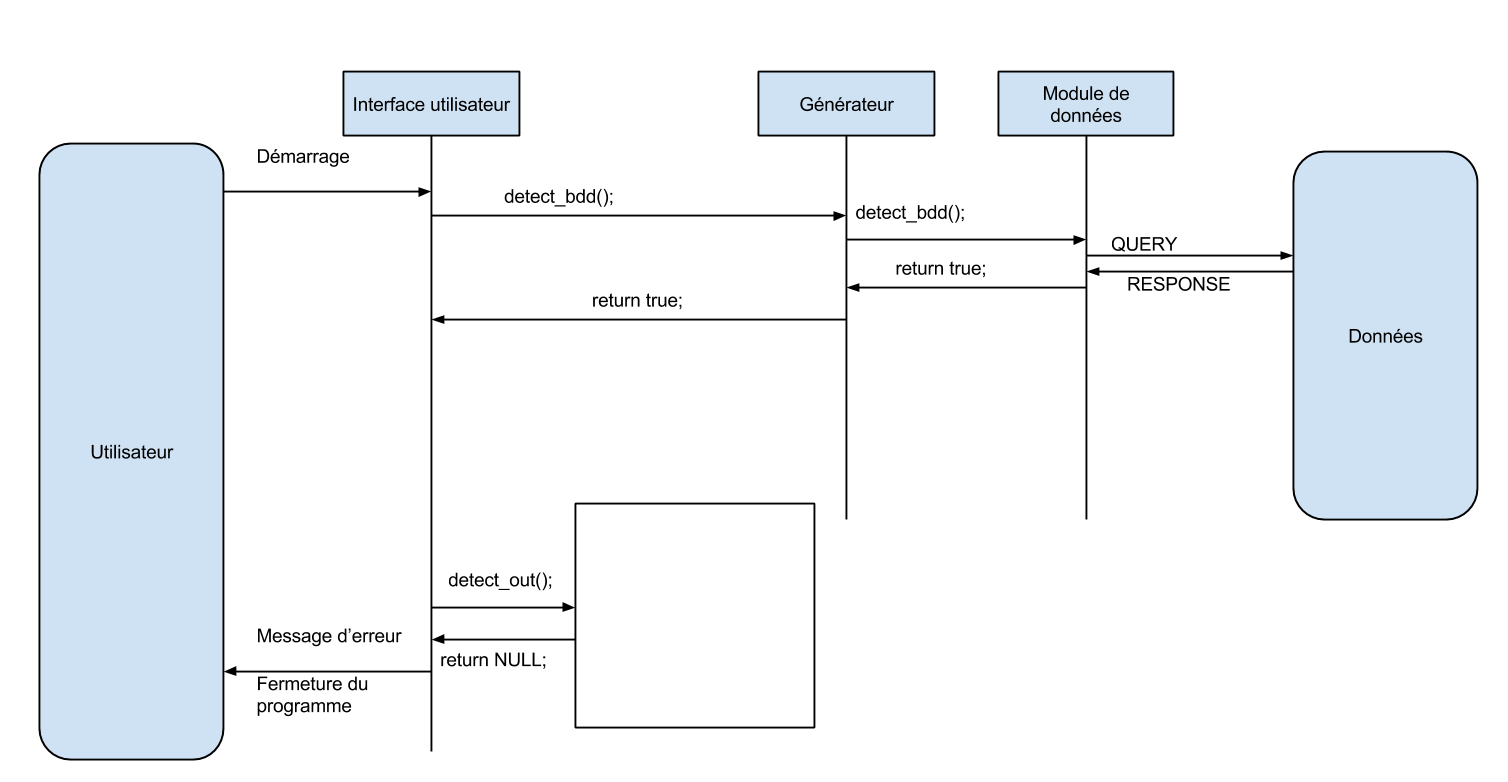
\includegraphics[width=\textwidth]{data/scenarii/demarrage_absence_sortie.png}
\caption{Absence de sorties disponibles lors de l'initialisation}
\end{figure}
 
\section{Génération}
\label{scenarii:gen}

\subsection{Génération fonctionnelle et satisfaisante}
\label{scenarii:gen:satis}

\begin{enumerate}
\item L'utilisateur décide de lancer la génération d'une playlist.
\item Le module d'interface utilisateur appelle le module de génération et 
lui transmet les paramètres entrés par l'utilisateur.
\item Le module de génération appelle le module de données et lui transmet 
une requête de morceaux satisfaisant les paramètres choisis par l'utilisateur.
\item Le module de données lance les requêtes SQL sur la base de données et
récupère les informations renvoyées.
\item Ces informations sont rendues au module de génération puis sont 
utilsées pour créer une liste de morceaux.
\item Le module de génération calcule la bonne similarité de la playlist.
\item Le module de génération renvoie la playlist ainsi crée à l'interface 
utilisateur qui la passe au module de sortie demandé.
\item Ce module génére la sortie et la rend directement à l'utilisateur en 
passant par l'interface.
\end{enumerate}

\begin{figure}[H]
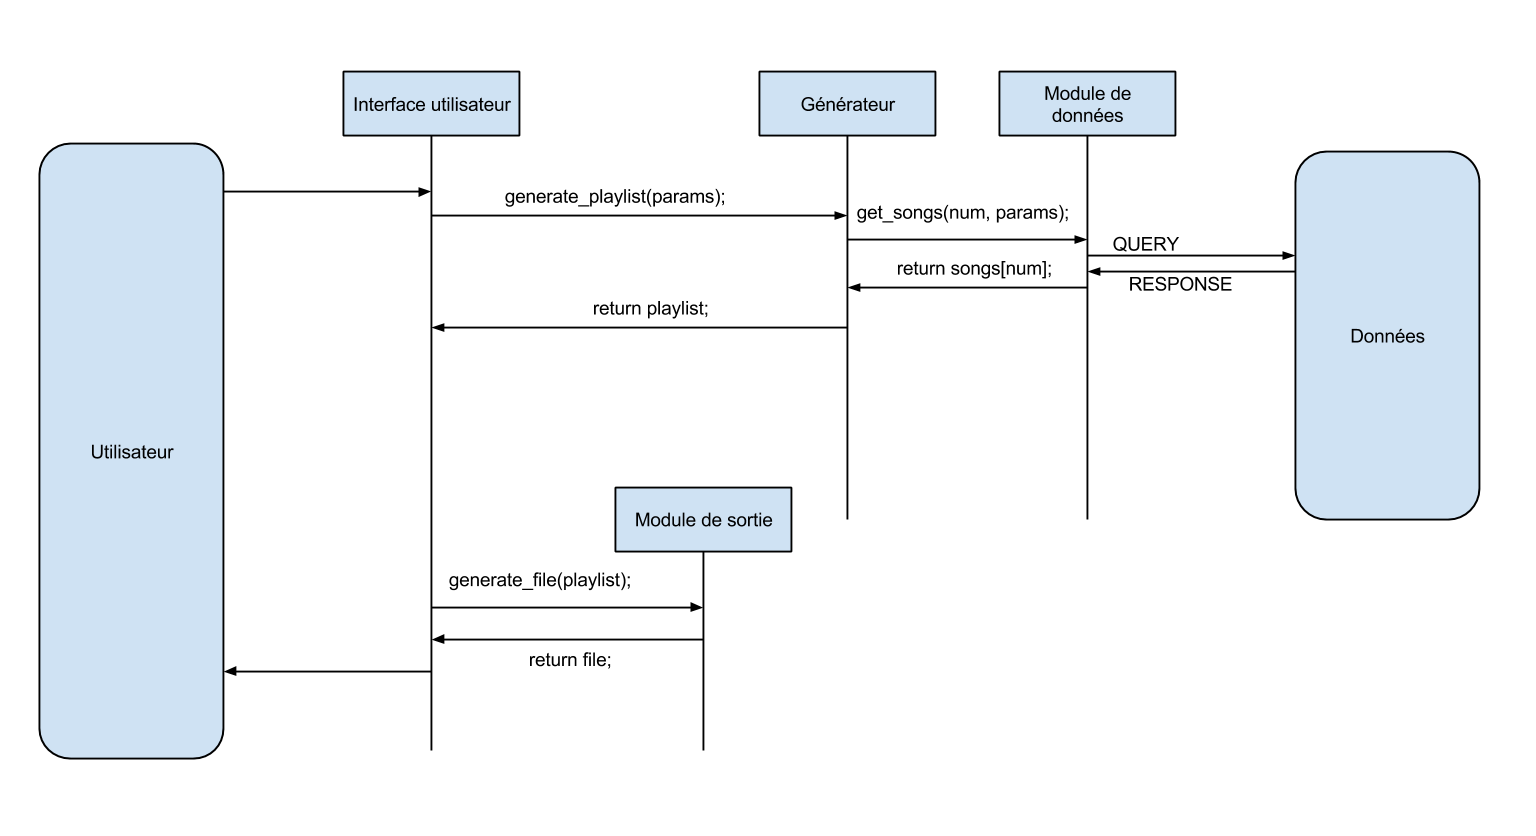
\includegraphics[width=\textwidth]{data/scenarii/generation_fonctionnel.png}
\caption{Génération de playlist réussie}
\end{figure}

\subsection{Génération non satisfaisante}
\label{scenarii:gen:nosatis}

\begin{enumerate}
\item L'utilisateur décide de lancer la génération d'une playlist.
\item Le module d'interface utilisateur appelle le module de génération et 
lui transmet les paramètres entrés par l'utilisateur.
\item Le module de génération appelle le module de données et lui transmet 
une requête de morceaux satisfaisant les paramètres choisis par l'utilisateur.
\item Le module de données lance les requêtes SQL sur la base de données et
récupère les informations renvoyées.
\item Ces informations sont rendues au module de génération puis sont 
utilsées pour créer une liste de morceaux.
\item Le module de génération calcule la bonne similarité de la playlist, 
mais celle ci ne répond pas aux attentes.
\item Le module de génération renvoie la playlist à l'IHM qui demande à 
l'utilisateur s'il veut affiner la recherche ou non.
\item Si oui, on lance une nouvelle génération en gardant la liste générée 
au passage précédent (On répète les étapes 3, 4, 5 et 6). Si non, on passe 
directement à l'étape suivante.
\item Le module de génération renvoie la playlist ainsi crée à l'interface 
utilisateur qui la passe au module de sortie demandé.
\item Ce module génére la sortie et la rend directement à l'utilisateur en 
passant par l'interface.
\end{enumerate}

\begin{figure}[H]
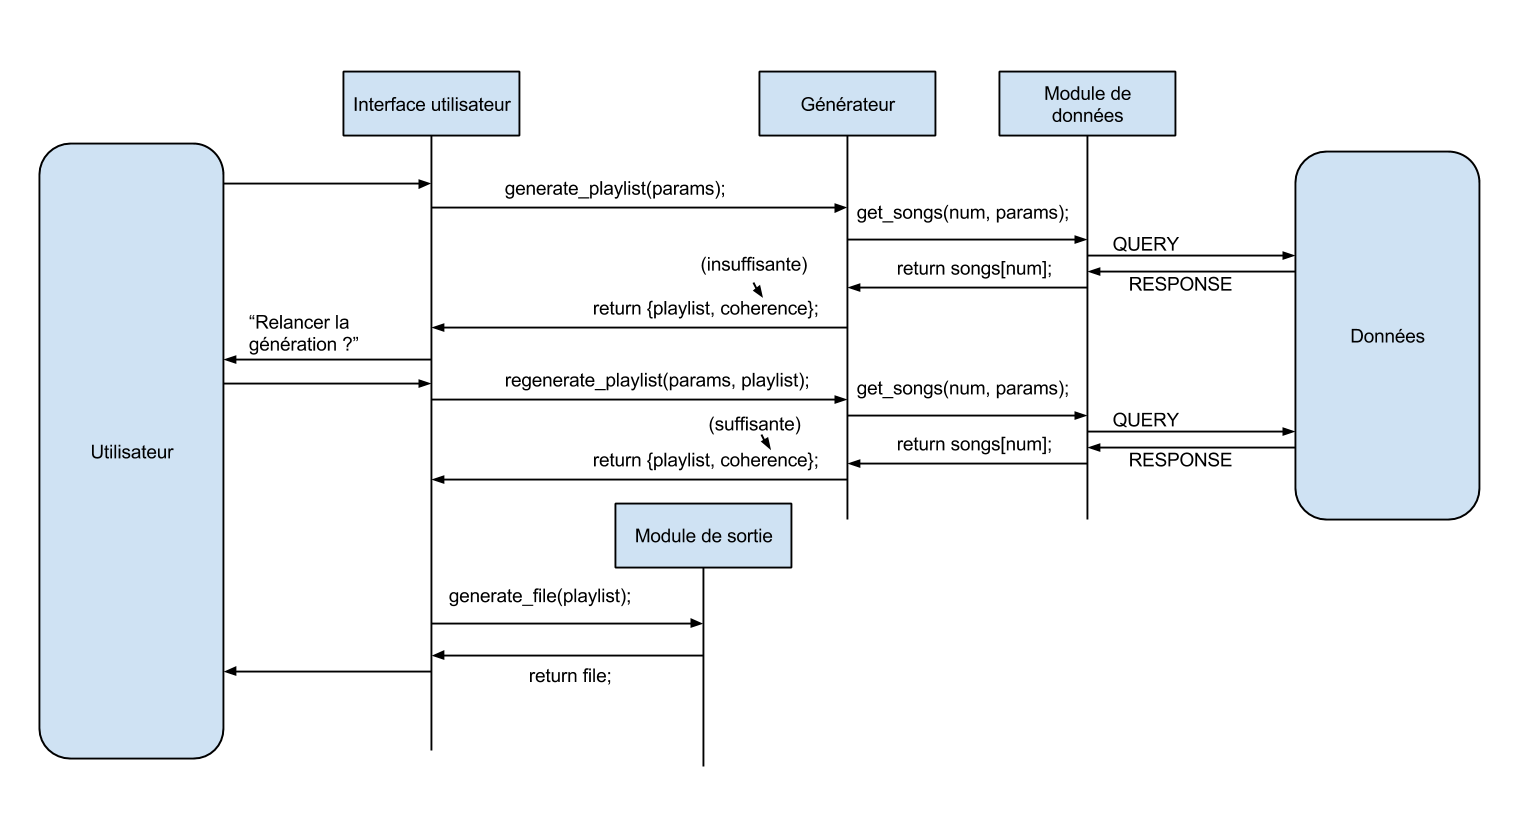
\includegraphics[width=\textwidth]{data/scenarii/generation_decevante.png}
\caption{Génération de playlist non staisfaisante, l'utilisateur relance la génération}
\end{figure}
 

\subsection{Génération incomplète}
\label{scenarii:gen:incomp}

\begin{enumerate}
\item L'utilisateur décide de lancer la génération d'une playlist.
\item Le module d'interface utilisateur appelle le module de génération et 
lui transmet les paramètres entrés par l'utilisateur.
\item Le module de génération appelle le module de données et lui transmet 
une requête de morceaux satisfaisant les paramètres choisis par l'utilisateur.
\item Le module de données lance les requêtes SQL à la base de données et
récupère les informations, mais il n'y a pas assez de morceaux correspondant 
aux critères demandés par l'utilisateur.
\item Ces informations sont rendues au module de génération puis sont 
utilsées pour créer une liste de morceaux.
\item Le module de génération calcule la bonne similarité de la playlist.
\item Le module de génération renvoie la playlist ainsi crée à l'interface 
utilisateur.
\item L'IHM avertit l'utilisateur que la playlist est incomplète avant de 
passer la playlist au module de sortie demandé.
\item Ce module génére la sortie et la rend directement à l'utilisateur en 
passant par l'interface.
\end{enumerate}

\begin{figure}[H]
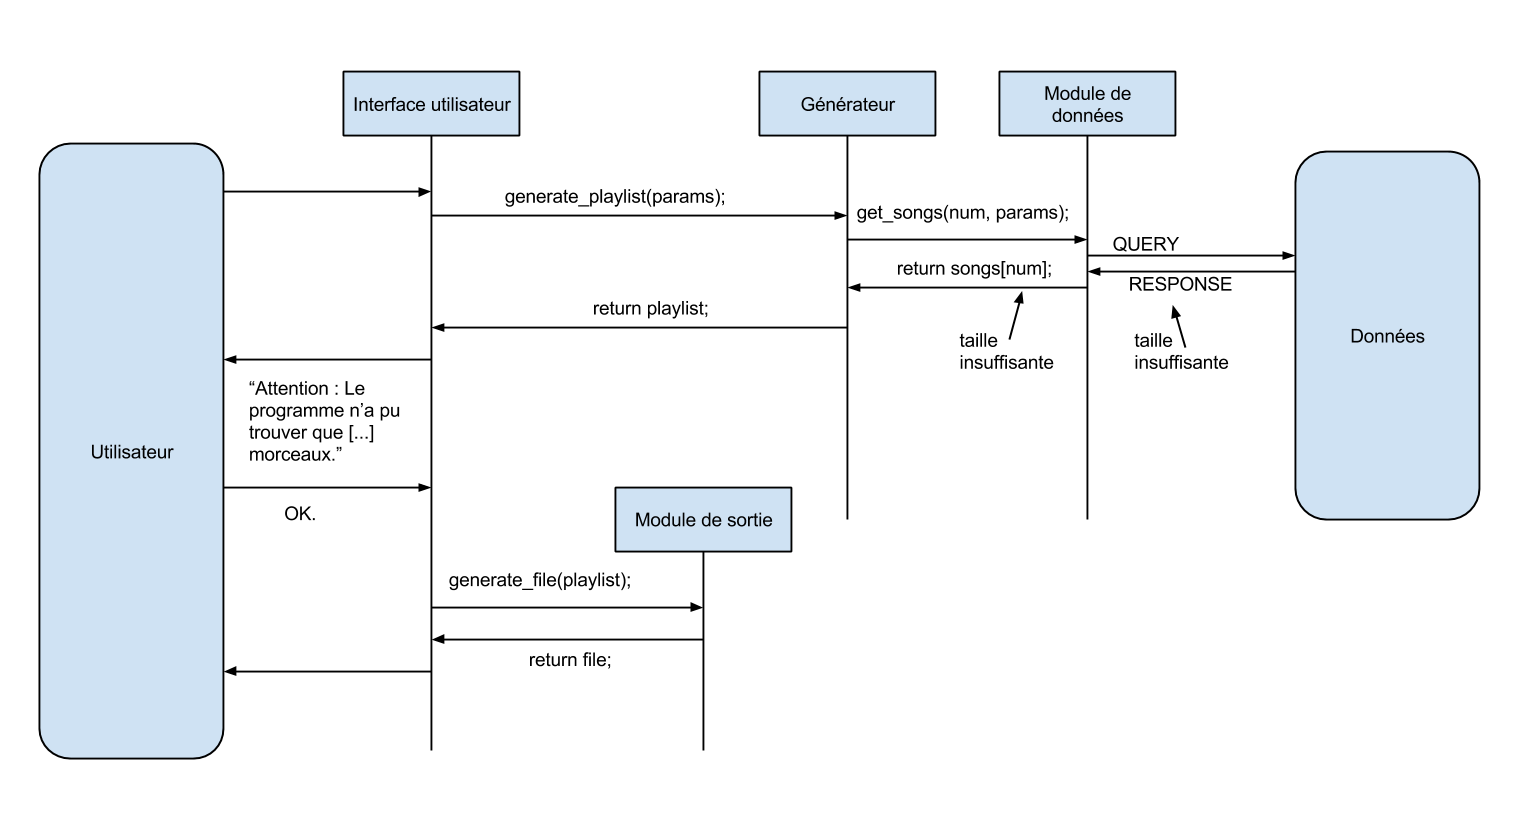
\includegraphics[width=\textwidth]{data/scenarii/generation_incomplete.png}
\caption{Génération terminée mais incomplète, on avertit l'utilisateur}
\end{figure}
 

\subsection{Absence de données répondant aux paramètres}
\label{scenarii:gen:nodata}

\begin{enumerate}
\item L'utilisateur décide de lancer la génération d'une playlist.
\item Le module d'interface utilisateur appelle le module de génération et 
lui transmet les paramètres entrés par l'utilisateur.
\item Le module de génération appelle le module de données et lui transmet 
une requête de morceaux satisfaisant les paramètres choisis par l'utilisateur.
\item Le module de données lance les requêtes SQL à la base de données mais 
ne récupère pas d'informations : il n'y a pas de morceaux correspondants aux 
critères demandés par l'utilisateur.
\item Le module de génération renvoie une liste vide à l'interface 
utilisateur.
\item L'IHM avertit l'utilisateur que la requête ne renvoie aucune 
information et qu'aucune playlist ne peut être générée.
\end{enumerate}

\begin{figure}[H]
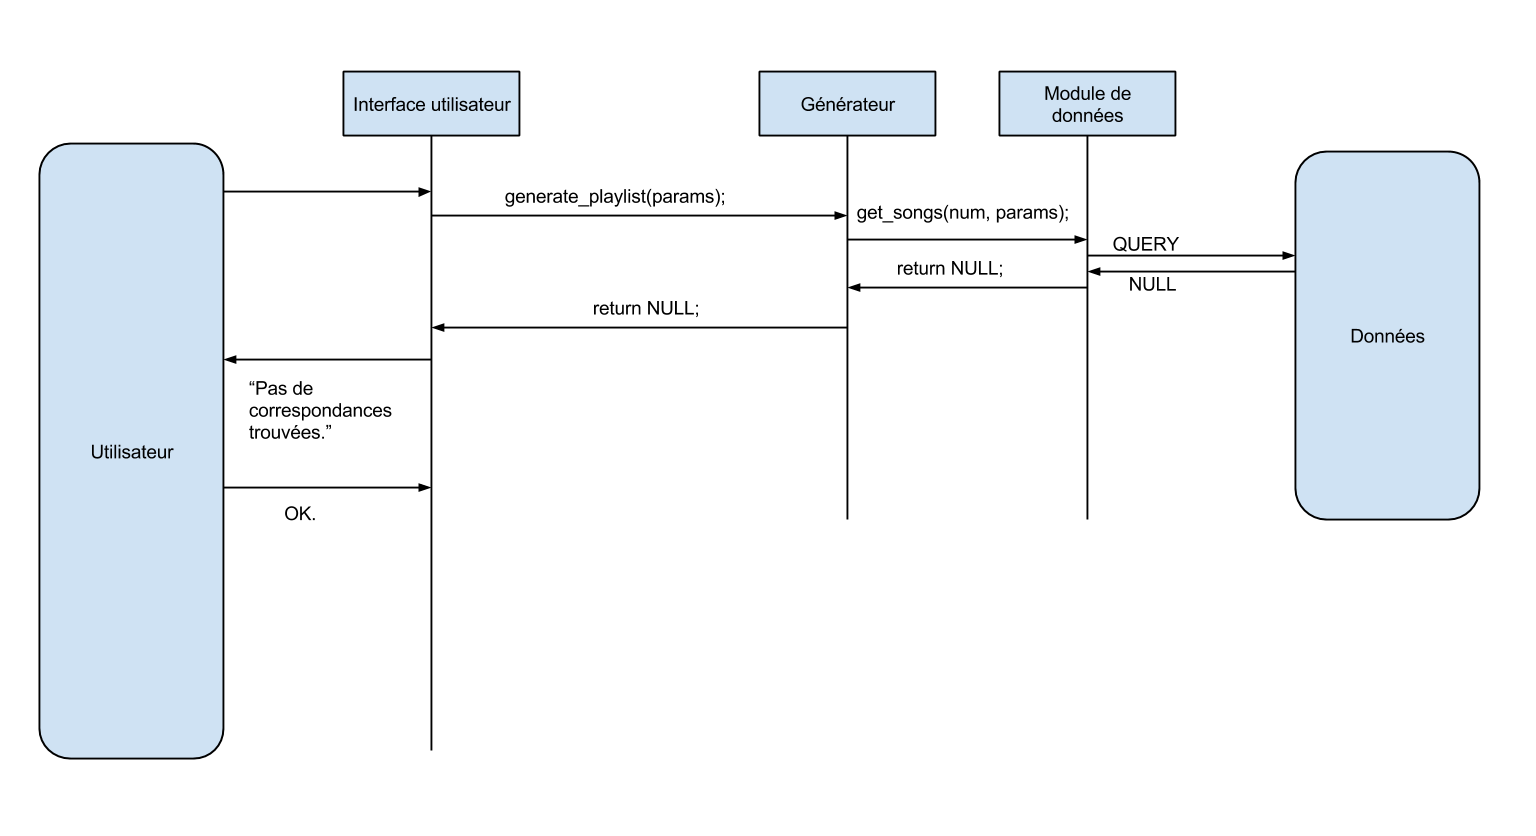
\includegraphics[width=\textwidth]{data/scenarii/generation_nulle.png}
\caption{Génération impossible, il n'y a pas de morceaux correspondants à la requête}
\end{figure} % Scénarios d'utilisation

\chapter{Architecture}

\section{Architecture des modules}
\label{archi:modules}

\subsection{Interface Utilisateur}
\label{archi:modules:iu}

L'Interface Utilisateur (UserInterface) se charge de faire le lien entre
l'utilisateur et le programme. Sa fonction principale est de lancer une
génération de playlist en appelant la fonction \texttt{generate} du module de 
génération. Lors de l'appel à cette fonction, les informations rentrées par 
l'utilisateur sont transmises en paramètres. Lors du lancement du programme,
 une fonction d'initialisation est lancée. Cette dernière permet d'assurer 
 la présence de la base de données ainsi que du, ou des, module(s) de sortie.

\subsection{Générateur}
\label{archi:modules:generateur}

Le module de génération (lui-même composé de 3 sous-modules: Generator, 
SimilarityEngine et FeedbackEngine) s'occupe de la création de la playlist. 
L'interface utilisateur appelle toutes les fonctions du sous-module 
Generator, et celui-ci appelle à son tour toutes les fonctions des deux 
autres sous-modules. La fonction \texttt{initialization} sert à vérifier la 
présence de base de données lors du démarrage du programme. 

La fonction \texttt{generate} sert à générer la playlist d'après les options 
passées via l'interface utilisateur. Elle effectuera un appel à la fonction 
\texttt{select} du module de données afin de récupérer un ensemble fini de morceaux.
 La fonction \texttt{regenerate} est utilisée dans la situation particulière où 
 l'utilisateur se voit proposer de faire une nouvelle génération dans le cas 
 où la génération précédente est jugée non satisfaisante (voir le dossier 
 d'Analyse de besoins). Cette fonction prend donc les options en paramètres 
 et récupère la précèdente playlist générée dans le but de l'améliorer.

Le sous-module SimilarityEngine sert à calculer la similarité entre deux 
morceaux afin de vérifier la cohérence et la validité de la playlist. Le 
sous-module FeedbackEngine permet de communiquer avec l'interface 
utilisateur pour apporter un visuel de la progression de la génération afin 
d'informer l'utilisateur de l'avancement de la création, et l'aider à 
patienter.

\subsection{Module de données}
\label{archi:modules:donnees}

Le module de données (SQLiteDatabase) a pour objectif d'assurer la 
communication entre le module de génération et la base de données utilisée. 
Sa principale fonctionnalité est d'effectuer une séléction dans la base de 
données en fonction du nombre de chansons souhaité et des paramètres de 
séléction entrés par l'utilisateur. Cette opération se fait grâce à la 
fonction \texttt{select}. De plus, lors du lancement du programme, une 
fonction d'initialisation est appellée afin de certifier la présence de la 
base de données.

\subsection{Module de sortie}
\label{archi:modules:sortie}

Le module de sortie (ici TextOutput) est en charge de fournir à 
l'utilisateur un moyen de récuperer le résultat de la génération demandée. 
Ce module (ainsi que tous les modules de sortie pouvant être crées) devront 
respecter l'interface OutputStrategy pour pouvoir être utilisés sur le 
programme. Dans le cas du module TextOutput, le résultat obtenu sera mis 
sous la forme d'un fichier texte contenant les titres des différents 
morceaux de la playlist. Cette fontionnalité est assurée par la fonction 
\texttt{format} à laquelle on passe la playlist générée en paramètre.

\section{Structures de données}
\label{archi:structures}

\subsection{Morceau}
\label{archi:structures:morceau}

Un morceau (Track) est la structure principale du programme. Cette dernière 
peut être utilisée tant pour décrire un morceau que pour décrire des 
paramètres (certains paramètres seront utilisés uniquement dans le premier 
cas). Les paramètres sont triés dans deux sous-sections (signal\_data et 
context\_data) dans un soucis de visibilité, à l'exception d'un \textit{id} 
qui concerne l'identifiant dans la base de données du morceau (utilisé pour 
éviter des duplications).

\subsubsection{Données signal}
\label{archi:structures:morceau:signal}

Les données signal, représentées par la structure SignalData, sont 
l'ensemble des valeurs correspondant aux déscripteurs audio du morceau, à 
savoir: le rythme, l'énergie et la tonalité (\textit{rythme}, \textit{energy}
 et \textit{tonality}). Ces valeurs sont exprimées par des nombres flottants 
 compris entre 0 et 1.

\subsubsection{Données de contexte}
\label{archi:structures:morceau:contexte}

Les données de contexte sont représentées par la structure ContextData, qui 
contient les informations sur le morceau qui ne sont pas relatives au 
signal : elles décrivent le contexte culturel du morceau. Ces informations 
sont :  un score de popularité exprimé par un nombre flottant compris entre 
0 et 1, l'artiste qui est à l'origine du morceau et l'album sur lequel il 
se trouve.

\subsubsection{Informations sur l'artiste et l'album}
\label{archi:structures:morceau:artiste}

Les informations sur l'artiste (Artist) contiennent un identifiant (qui 
dépendra de la base de données), le nom de l'artiste interprète du morceau 
qui sera stocké dans une chaîne de caractères, ainsi qu'une liste d'artistes 
similaires.

L'album contient lui aussi un identifiant, son nom (qui est utilisé par le 
module de sortie dans le cas où c'est nécessaire), l'artiste de l'album 
(pouvant différer de celui du morceau dans le champ \textit{artist}, par 
exemple dans le cas d'une collaboration avec une autre personne), et l'année 
de sortie.

Ces deux sections appartienent aux données de contexte.

\subsection{Playlist et échantillon de morceaux}
\label{archi:structures:playlist}

La Playlist et l'échantillon de morceaux sont deux listes de morceaux. La 
première est remplie par le module de données, et la deuxième par le 
générateur. La Playlist contient un booléen qui permet de renseigner la 
satisfaction ou non du résultat à l'interface utilisateur, afin de proposer, 
dans le cas où la playlist n'est pas satisfaisante, une nouvelle génération 
à l'utilisateur.

\subsection{Paramètres}
\label{archi:structures:param}

Les paramètres du programme entrés par l'utilisateur seront représentés et 
stockés sous la forme d'un morceau. Les champs non-utilisés par le programme 
seront ignorés, et les champs non-renseignés par l'utilisateur seront 
affectés à des valeurs spécifiques afin de signifier qu'elles ne sont pas 
utilisées : les champs de type \textit{string} seront vides, les champs de 
type \textit{float} auront la valeur 2 (puisque nous n'utilisons que des 
valeurs comprises entre 0 et 1), et les années de sortie de type 
\textit{int} seront mises à 0. % Architecture

\chapter{Implementation}
\section{Génération}
\label{impl:generation}

L'objectif du générateur étant d'assurer une similarité entre tous les
morceaux de la playlist mais surtout d'assurer la similarité des morceaux deux
à deux dans l'enchainement des morceaux il a été choisi d'implémenter notre
algorithme de génération sous forme itérative.

\subsection{Algorithme naïf}
\label{impl:selection:naif}

La première solution proposée pour implémenter la génération de playlist a été
de réaliser un algorithme glouton et naïf.\newline

L'algorithme est le suivant~:

\begin{enumerate}
\item Début.
\item Le premier morceau de la Pool devient le premier morceau de la Playlist.
\item Tant que la Playlist n'a pas la taille requise et que la Pool n'est pas
vide~:
  \begin{enumerate}
    \item On met le maximum de smilarité à 0.
    \item Pour chaque morceau t dans la Pool~:
      \begin{enumerate}
        \item On calcule le score de similarité entre t et le dernier morceau
        de la Playlist.
    \item Si le score de similarité est supérieur au score maximum~:
        \begin{enumerate}
        \item On remplace le score maximum par le nouveau score manimum.
        \item On enregistre le morceaux qui a le meilleur score de similarité.
        \end{enumerate}
        \end{enumerate}
        \item On ajoute le morceau qui a la similarité maximale à la fin de la
        Playlist actuelle.
    \end{enumerate}
    \item Si la similarité globale de la Playlist est suffisante~:
    \begin{enumerate}
    \item On marque la Playlist comme valide.
    \end{enumerate}
    \item Fin.
\end{enumerate}

Les résultats de cet algorithme sont bons mais il n'est cependant pas optimal.
En effet à chaque ajout de morceau dans la Playlist cet algorithme ne vérifie
pas la similarité du morceau testé avec tous les morceaux de la Playlist et
n'assure pas que le morceau après lequel il est ajouté est celui avec lequel
il a le plus grand score de similarité.


\subsection{Algorithme optimal}
\label{impl:selection:optimal}

Comme énoncé précedemment, le premier algorithme implémenté n'est pas optimal.
Il a donc été important de chercher un algorithme proposant une solution
optimale ou capable de s'en approcher.\newline

La solution trouvée est de considerer tous les morceaux de la Pool et d'en
constituer un graphe complet reliant tous les morceaux les uns aux autres. Les
arêtes seraient alors pondérées par le score de similarité entre les morceaux
situés à leurs extrémités. Une fois le graphe construit il faut appliquer un
algorithme capable de calculer le coût de tous les chemins de taille N (avec N
la taille souhaitée pour la Playlist).\newline

Un nouveau problème se pose alors~: Le calcul de similarité utilise les
informations contenues dans la base de données. Ne sachant pas la précision de
ces informations la question se pose alors de savoir s'il est pertinent
d'utiliser un algorithme de grande complexité et de chercher un résultat
optimal à partir de données non vérifiables.

\subsection{Optimisation}
\label{impl:selection:optimisation}

Suite à la question que pose l'utilisation d'un algorithme optimal, il a été
décidé que celui-ci ne serait pas implémenté et qu'il serait préférable
d'améliorer le résultat obtenu par l'algorithme naïf en y apportant une légère
optimisation.\newline

En effet la faiblesse de cet algorithme est de ne comparer les morceaux
restants dans la Pool qu'au dernier morceau ajouté dans la Playlist. Cette
dernière étant implémentée par une liste doublement chaînée il a alors été
décidé de comparer les éléments restants dans la Pool au dernier mais aussi au
premier élément de la Playlist afin d'augmenter les chances d'obtenir un
meilleur résultat.


\section{Similarité}
\label{impl:similarite}

Afin de conserver une cohérence avec la façon dont sont représentés les
différentes données autour des morceaux, il a été choisi de toujours ramener
le score de similarité calculé entre 0 et 1.

\subsection{Pattern strategy}
\label{impl:similatite:strategy}

Comme énoncé précédemment (c.f. Section
\ref{besoins:nfonc:perf:mod:similarity}) il a été choisi d'implémenter le calcul de similarité en suivant le pattern
strategy.\newline

Ce choix a été guidé par le fait que la base de données utilisée par notre
générateur pouvant être changée par l'utilisateur. Il faut donc pouvoir
facilement adapter notre calcul de similarité à une nouvelle base de données
afin d'assurer que le générateur conserve sa pertinence.

\subsection{Calcul de similarité naïf}
\label{impl:similarite:naif}

Dans un premier temps nous avons choisi d'implémenter un calcul de similarité
dit «~naïf~» afin d'assurer un fonctionnement minimal à notre générateur. 
Le but de ce calcul n'est pas d'être pertinent mais de permettre de valider
l'ordonnancement de plusieurs morceaux en fonction d'un seul critère.

Pour cette implémentation du calcul, on se base uniquement sur la différence
entre les années de sorties des albums dont sont extraits les morceaux à
laquelle est appliquée un logarithme décimal. L'utilisation du logarithme
décimal sert à considérer l'écart d'année entre les morceaux de façon
non-linéaire afin d'atténuer les variations trop importantes. Le calcul est
donc le suivant(avec date1 et date2 les années de sortie des albums des pistes
track1 et track2)~:

\begin{equation*}
  score(track1, track2) = log_{10}(date1 - date2)
\end{equation*}\newline

Enfin, pour ramener le score de similarité entre 0 et 1 on applique les
opérations suivantes en considérant un seuil en dessous duquel la différence
d'années est considérée négligeable~:

\begin{itemize}
\item score = 1, si le score est supérieur à 1. 
\item score = 0, si le score le score est inférieur au seuil.
\item on retourne (1 - score) afin que 0 représente une similarité nulle et 1
une similarité totale.
\end{itemize}

\subsection{Calcul de similarité complet}
\label{impl:similarite:complet}

Dans l'implémentation de ce calcul de similarité dit «~complet~», la formule
utilisée pour produire un score prend en compte plusieurs caractéristiques des
morceaux comparés. Ces caractéristiques sont extraites de la base de données
et sont les suivantes~:

\begin{itemize}
\item le rythme
\item l'énergie
\item la date de sortie de l'album dont est extrait le morceaux
\item le nom de l'artiste
\end{itemize}

On peut imaginer la répartition de chaque morceau dans un repère à 4
dimensions où chacun des axes représente une de ces quatre caractéristiques.
Le score de similarité est alors calculé en faisant une moyenne de la
variation entre les deux morceaux sur chacun de ces axes.

Afin d'établir un ordre d'importance entre ces caractéristiques on décide de
pondérer cette moyenne avec les facteurs suivants~:

\begin{itemize}
\item le rythme compte pour 40\%
\item l'énergie compte pour 30\%
\item la date de sortie de l'album compte pour 20\%
\item le nom de l'artiste compte pour 10\%
\end{itemize}

Ces facteurs de pondération on été choisis de façon à ce que les données
signal representent 70\% du score de similarité et les données contextuelles
les 30\% restants.

\subsubsection{Rythme et énergie}
\label{impl:similarite:complet:rhythm}

La variation entre les deux morceaux sur les axes représentant le rythme et
l'énergie se fait de façon classique en inversant le résultat pour toujours
considérer 0 comme une similarité nulle et 1 comme une similarité totale comme
suit(avec rhythm1, energy1, rhythm2 et energy2 respectivement les rythmes et
énergies des deux morceaux comparés) ~:

\begin{align}
  \Delta Rhythm = 1 - |rhythm1 - rhythm2|\\
  \Delta Energy = 1 - |energy1 - energy2|
\end{align}

\subsubsection{Date de sortie de l'album}
\label{impl:similarite:complet:date}

La variation entre les dates de sorties des albums dont sont extraits les deux
morceaux est calculée de la même façon que dans le calcul de similarité naïve.
(c.f \ref{impl:similarite:naif})

\subsubsection{Nom d'artiste}
\label{impl:similarite:complet:name}

On considère que deux morceaux du même artiste ont de grandes chances d'être
similaires. Cette carectèristique étant faiblement pondéré dans le calcul de
similarité on peut définir la variation sur le nom d'artiste comme suivant~:

\begin{align}
  \Delta Artist = \text{1, si artist1 = artist2.}\\
  \Delta Artist = \text{0, sinon.}
\end{align}

\section{Module de données SQLite}
\label{implementation:sqlite}

L’implémentation du module de données SQLite (classe \texttt{SQLiteDatabase})
à été réalisée en utilisant la bibliothèque sqlite3
\footnote{http://www.sqlite.org/about.html}. Elle permet une interface avec les
fichiers sqlite. Elle est écrite en C, mais cela n'a pas posé de problème
particulier.

L’implémentation de la sélection dans le module SQLite est divisée en plusieurs
phases~:
\begin{description}
  \item[La création de la requête~:] au format SQL, qui doit prendre en compte
  les options passsés en paramètre à \texttt{select}. Des buffer de chaîne de
  caractères ont été utilisés, permettant de meilleures performances. L'usage de
  la fonction \texttt{random} avec la directive \texttt{ORDER BY}, permet la
  sélection aléatoire.

  \item[Execution et traitement de la requête~:] La requête est exécutée, puis
  chaque ligne renvoyée par la base de données SQLite est transformé en une
  piste, qui est ajouté à une liste temporaire.

  \item[Ajout des artistes similaires~:] il faut demander à la base de donnée
  quels sont les artistes similaires pour chaque piste sélectionnée. Le procédé
  est relativement similaire à la phase précédente, mais est exécutée pour
  chaque piste.

  \item[Copie des pistes dans un \texttt{Trackpool}~:] Pour finir la liste
  temporaire est copiée dans un \texttt{Trackpool}, qui sera retourné par la
  fonction. La liste temporaire était nécéssaire, car la \texttt{Trackpool} ne
  permet pas de modifier ses éléments.
\end{description}
 % Choix d'implementation

\chapter{Tests}

\section{Tests Unitaires}
\label{tests:unitaires}

\subsection{Module SQLite}
\label{tests:unitaires:sqlite}

\subsubsection{Sélection aléatoire}
\label{tests:unitaires:sqlite:random}

Ce test unitaire vérifie que deux sélections totalement aléatoires (toutes les
options non renseignées) sont bien différentes, comme demandé dans la
spécification. Son déroulement est assez simple, on réalise deux sélections avec
une liste d'options vide, puis on compare les deux ensembles sélectionnés.
Pour cela on cherche les pistes du premier ensemble sélectionné dans le second
ensemble. Si un élément du premier ensemble n'est pas présent dans le second,
les ensemble sont différents et le test est réussi.

\subsubsection{Filtrage par année}
\label{tests:unitaires:sqlite:annee}

Ce test vérifie que le filtrage des morceau par année fonctionne. Il choisit les
années de sélection entre 1990 et 2000, car c'est une période suffisamment
présente dans la MSD. Ensuite il faut analyser les pistes de l'ensemble
sélectionné et vérifier que leur année de sortie est bien comprise dans
l'intervalle d'années précisée. Si tous les morceaux passent ce test, le test
est une réussite.

\subsubsection{Filtrage par popularité}
\label{tests:unitaires:sqlite:popularite}

% TODO

\section{Tests de qualité de la playlist}
\label{tests:qualite}

La qualité d'une playlist est très subjective. Cependant dans notre projet cette
qualité est assuré par notre algorithme de similarité. Il fallait donc des tests
pour attester de la qualité de cette similarité. Les test qui vont suivre ne
sont pas des test binaires (seulement réussit ou raté), mais des outils
permettant d'analyser la qualité d'un algorithme de similarité.

\subsection{Test de cohérence : Technique du «~Grand Fossé~»}
\label{tests:qualite:coherence-fosse}

Ce test permet de tester la \emph{cohérence} de la playlist. Il repose sur la
génération de deux ensembles de morceaux très différents qui constitueront les
données dans lesquelles les morceaux seront sélectionnées, On crée donc
artificiellement un «~fossé~» entre les morceaux. On n'utilise donc pas la
«~vraie~» base de données. Nous avons choisit de simuler deux ensembles très
différents selon les critères suivant~:

\begin{description}

\item[Hard Métal (rapide et puissant)~:] \hfill
\begin{itemize}
  \item rythme entre 0.75 et 1.0
  \item energie entre 0.85 et 1.0
\end{itemize}

\item[Aerial Ambient (lent et léger)~:] \hfill
\begin{itemize}
  \item rythme entre 0.0 et 0.2
  \item énergie entre 0.0 et 0.35
\end{itemize}

\end{description}

Après avoir généré ces deux ensemble de morceaux, il suffit de générer une
playlist avec la base de donnée résultante. Si des morceaux des deux ensembles
sont dans la playlist la qualité de la similarité est à revoir.

Il est important de noter que la taille de la playlist générée est importante,
ainsi que le rang du premier morceau non valide. En effet, plus la playlist est
grande, plus le risque de traverser le fossé est grand. On fixera donc la taille
de la playlist à générer à 1000 morceaux, ce qui est largement suffisant pour
tester la robustesse de la similarité (la plupart des playlists générées ne
dépassant pas 100 pistes). De plus, un morceau non valide à un rang élevé (par
exemple la 800e piste) est moins critique pour la qualité de la playlist qu'un
rang bas (par exemple 10e piste).

Il faut donc prendre en compte ces éléments dans la mise en place d'un score de
réussite au test. On calculera ce score en fonction du rang du morceau non
valide dans la playlist. Une playlist sans morceau invalide aura un score de
100\%.

On utilise donc la formule suivante pour calculer le score du test, n
correspondant au rang de la piste invalide, et N à la taille de la playlist
générée (généralement 1000)~:

\begin{equation*}
  score(n) = log_{10}(1 + \frac{n}{N} * 9)
\end{equation*}

Grâce à cette formule, le score atteint 70\% à la moitié de la playlist (500).
Ainsi les premier rang sont plus important pour le score que les derniers.

En réalisant ce test de multiples fois et en faisant la moyenne des scores
obtenus on obtient un aperçu assez clair de la qualité de la cohérence induite
par notre calcul de similarité.

\subsection{Test de variation : Technique de la «~Passerelle~»}
\label{tests:qualite:variation-passerelle}

Ce test permet de tester la \emph{variation} de la playlist. Pour cela il
utilise les deux ensembles extrêmes utilisés par le test de cohérence, en 
ajoutant un troisième ensemble qui jouera le rôle de passerelle entre les
deux autres.

L'ensemble passerelle sera généré pour contenir des morceaux qui comblent le
vide entre les deux ensembles extrêmes~:

\begin{itemize}
  \item rythme entre 0.2 et 0.75
  \item énergie entre 0.35 et 0.85
\end{itemize}

Tout l'enjeu du test est qu'une playlist qui commence par un morceau du premier
ensemble extrême contienne un morceau de l'autre ensemble extrême, le troisième
ensemble servant de pont, grâce à la variation introduite dans le calcul de
similarité.

Pour que le test soit viable, l'ensemble passerelle doit être construit de
manière réfléchie~: la distance entre les morceaux la composant doit être faible,
il ne faut pas qu'il y ait de discontinuité dans les descripteurs, sinon la
passerelle ne marchera pas.

Comme pour le test de cohérence on génère des playlists de 1000 morceaux.
Cependant, cette fois ci le score doit prendre en compte deux événements~:
\begin{description}
  \item[Le rang du premier morceau de la passerelle~:] car c'est la première
  étape, un algorithme de similarité qui n'arrive pas à ce stade prend très peu
  en charge la variation.
  \item[Le rang du premier morceau de l'autre ensemble extrême~:] c'est
  l'aboutissement du test. Il est important de noter qu'un rang trop bas indique
  Un manque de cohérence pour la similarité.
\end{description}

Le meilleur moyen de conduire ce test est encore une fois de le répéter. On
obtiens ainsi une moyenne des rangs d'atteinte de la passerelle et de ceux
d'atteinte de l'autre extrême. % descriptions des tests

% \chapter*{Conclusion}

% TODO: Conclusion

\backmatter

% Bibliographie : désactiver pour l'instant
\bibliographystyle{plain}
\bibliography{memoire}

% Liste des schémas
\listoffigures

\end{document}
